% Proposta H (12/11/2026, pedido do autor): a G sem as faixas, com mais espaço
% entre as caixas, a seta do "sim" mais longa e margem branca para print. Os dois
% ramos nascem do mesmo ARIMA e se juntam na ordem, que recebe o lado de um e o
% tamanho do outro (as duas setas finais têm esses nomes). O losango fica no ramo
% do risco e só recebe a volatilidade. Sem fórmula. Exportada também em PNG
% (fig-integracao-h.png, 300 dpi) para o autor copiar. Fora do TG até decidir.
\documentclass[11pt,border=14pt]{standalone}
\usepackage[T1]{fontenc}
\usepackage[utf8]{inputenc}
\usepackage{mathptmx}
\usepackage{tikz}
\usetikzlibrary{arrows.meta,positioning,calc,shapes.geometric}
\tikzset{
  seta/.style={-{Stealth[length=2.4mm]}, semithick},
  caixa/.style={rectangle, draw, semithick, fill=gray!10, rounded corners=2pt,
                align=center, minimum width=44mm, minimum height=11mm, font=\small},
  dado/.style={trapezium, trapezium left angle=75, trapezium right angle=105, draw,
               semithick, fill=white, align=center, minimum height=10mm, font=\small,
               trapezium stretches body},
  decisao/.style={diamond, draw, semithick, fill=white, aspect=1.9, align=center,
                  inner sep=0.5pt, font=\small},
  pergunta/.style={font=\small\itshape},
  pequeno/.style={font=\footnotesize},
  rotulo/.style={font=\footnotesize\itshape, fill=white, inner sep=2pt},
}
\begin{document}
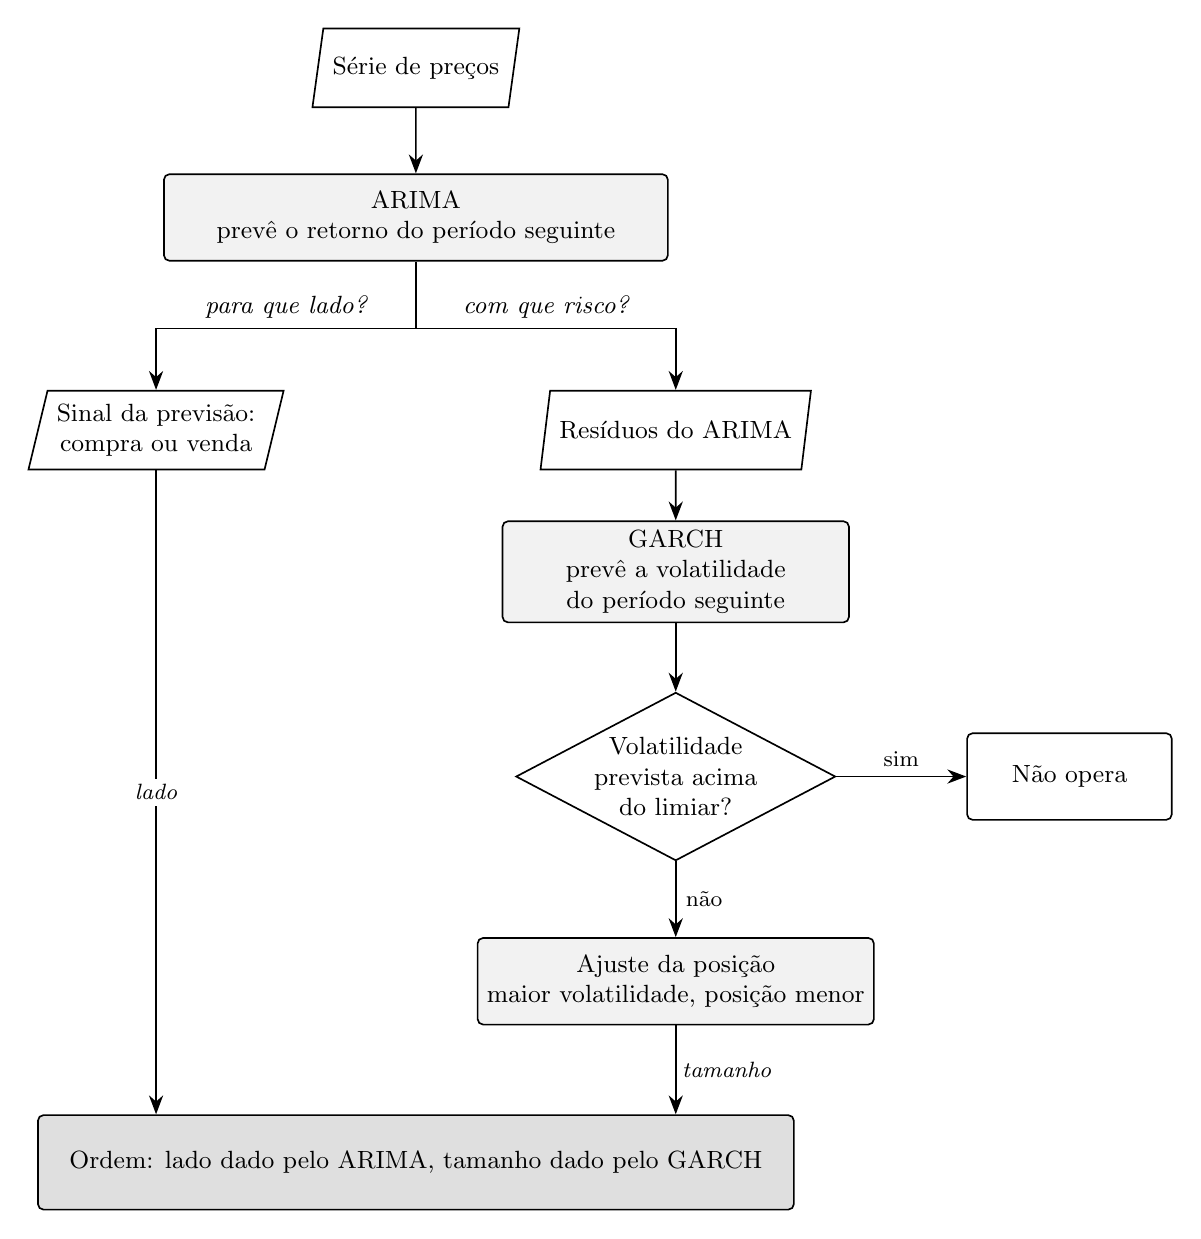
\begin{tikzpicture}
  \def\xa{-3.3}  % ramo da direção
  \def\xg{3.3}   % ramo do risco

  \node[dado] (ent) at (0,0) {Série de preços};
  \node[caixa, minimum width=64mm] (arima) at (0,-1.9) {ARIMA\\prevê o retorno do período seguinte};

  % ramo da direção
  \node[dado] (dir) at (\xa,-4.6) {Sinal da previsão:\\compra ou venda};

  % ramo do risco
  \node[dado] (res) at (\xg,-4.6) {Resíduos do ARIMA};
  \node[caixa] (garch) at (\xg,-6.4) {GARCH\\prevê a volatilidade\\do período seguinte};
  \node[decisao] (lim) at (\xg,-9.0) {Volatilidade\\prevista acima\\do limiar?};
  \node[caixa, minimum width=26mm, fill=white] (veto) at (\xg+5.0,-9.0) {Não opera};
  \node[caixa] (tam) at (\xg,-11.6) {Ajuste da posição\\maior volatilidade, posição menor};

  % a integração: os dois ramos se juntam na ordem
  \node[caixa, fill=gray!25, minimum width=96mm, minimum height=12mm] (ord) at (0,-13.9)
    {Ordem: lado dado pelo ARIMA, tamanho dado pelo GARCH};

  % setas
  \draw[seta] (ent) -- (arima);
  \coordinate (div) at ($(arima.south)+(0,-0.85)$);
  \draw[semithick] (arima.south) -- (div);
  \draw[seta] (div) -| (dir.north);
  \draw[seta] (div) -| (res.north);
  \draw[seta] (res) -- (garch);
  \draw[seta] (garch) -- (lim);
  \draw[seta] (lim) -- node[above, pequeno]{sim} (veto);
  \draw[seta] (lim) -- node[right, pequeno]{não} (tam);
  \draw[seta] (dir.south) -- node[rotulo]{lado} (dir.south |- ord.north);
  \draw[seta] (tam.south) -- node[rotulo, right, fill=none]{tamanho} (tam.south |- ord.north);

  % as duas perguntas, sobre a divisão dos ramos
  \node[pergunta, above] at ($(div -| \xa,0)!0.5!(div)$) {para que lado?};
  \node[pergunta, above] at ($(div)!0.5!(div -| \xg,0)$) {com que risco?};
\end{tikzpicture}
\end{document}
